% coding:utf-8

%----------------------------------------
%FOSADSVB, a LaTeX-Code for a summary of digital signal processing
%Copyright (C) 2015, Mario Felder & Michi Fallegger

%This program is free software; you can redistribute it and/or
%modify it under the terms of the GNU General Public License
%as published by the Free Software Foundation; either version 2
%of the License, or (at your option) any later version.

%This program is distributed in the hope that it will be useful,
%but WITHOUT ANY WARRANTY; without even the implied warranty of
%MERCHANTABILITY or FITNESS FOR A PARTICULAR PURPOSE.  See the
%GNU General Public License for more details.
%----------------------------------------

\chapter{Optimale Lineare Filter}
\section{Wiener Filter}
Ist optimal im mittleren quadratischen Fehler.\\
\\
Zurückgewonnenes Signal $\hat{s}[n+D]$.
\begin{itemize}
	\item \textit{Smoothing:} Bei $D<0$ ist der Sinn Rauschen vom Signal zu
	eliminieren und eine Verzögerung von $-D$ in kauf zu nehmen. Für jedes Sample
	erzeugt der Filter eine Schätzung auf der Basis von $M+1$ Sampels von $y[n]$
	\item \textit{Filtering:} Bei $D=0$ ist die Absicht das Signal $s[n]$ zu regenerieren.
	Es werden keine Verzögerungen erzeugt, da die Abschätzung aufgrund des 
	aktuellen und vergangenen Werten gemacht wird.
	\item \textit{Prediction:} Bei $D>0$ will das Signal vorhergesagt werden.
\end{itemize} 
\begin{center}
	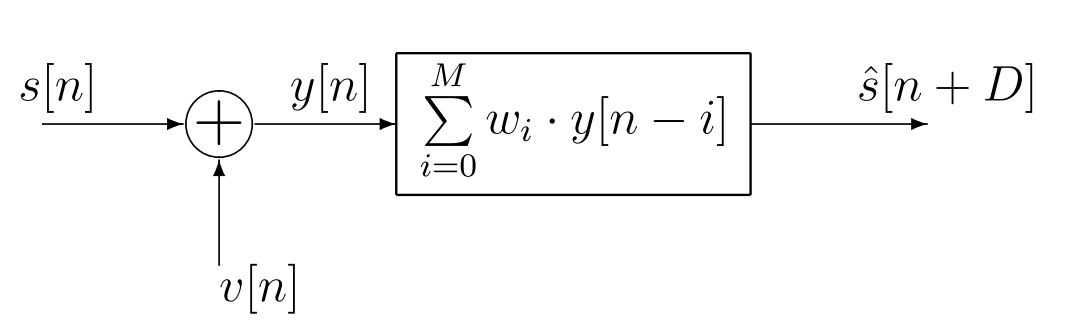
\includegraphics[scale=.7]{./images/wiener_filter}
\end{center}
Filterausgang:
\[ \hat{s}[n+D] = \sum_{i=0}^{M}w_i\cdot y[n-i] \]
Fehler:
\[ \hat{s}[n+D] - s[n+D] \]
Um die optimalen Parameter $w_i$ zu finden muss der Gradient auf Null gesetzt 
werden
\[ \sum_{i=0}^{M}\tilde{w}_i \cdot \gamma_{yy}[m-i] = \gamma_{sy}[m+D] \qquad
	m=0,1,...,M \]
mit der Autokorrelation des Filter Eingangs:
\[ \gamma_{yy} = E\{ y[n] \cdot y^*[n-m] \} \]
und der Kreuzkorrelation
\[ \gamma_{sy} = E \{ s[n] \cdot y^*[n-m] \} \]
~\\
Winer-Hopf Gleichung
\[ \textbf{R}_{yy} = \begin{bmatrix}
	\gamma_{yy}[0]	& \gamma_{yy}[-1]	& \ldots	& \gamma_{yy}[-M]\\
	\gamma_{yy}[1]	& \gamma_{yy}[0]	& \ldots	& \gamma_{yy}[1-M]\\
	\vdots			& \vdots			&			& \vdots\\
	\gamma_{yy}[M]	& \gamma_{yy}[M-1]	& \ldots	& \gamma_{yy}[0]
\end{bmatrix}\]
\[ \textbf{r}_{sy} = \begin{bmatrix}
	\gamma_{sy}[D]\\
	\gamma_{sy}[D+1]\\
	\vdots\\
	\gamma_{sy}[D+M]
\end{bmatrix} \qquad
  \tilde{\textbf{w}} = \begin{bmatrix}
	\tilde{w}_0\\
	\tilde{w}_1\\
	\vdots\\
	\tilde{w}_M
\end{bmatrix} \]
Die optimalen Filterkoeffizienten sind gegeben Durch:
\[ \tilde{\textbf{w}} = \textbf{R}_{yy}^{-1}\textbf{r}_{sy} \]